\begin{figure}[t!]
\begin{center}
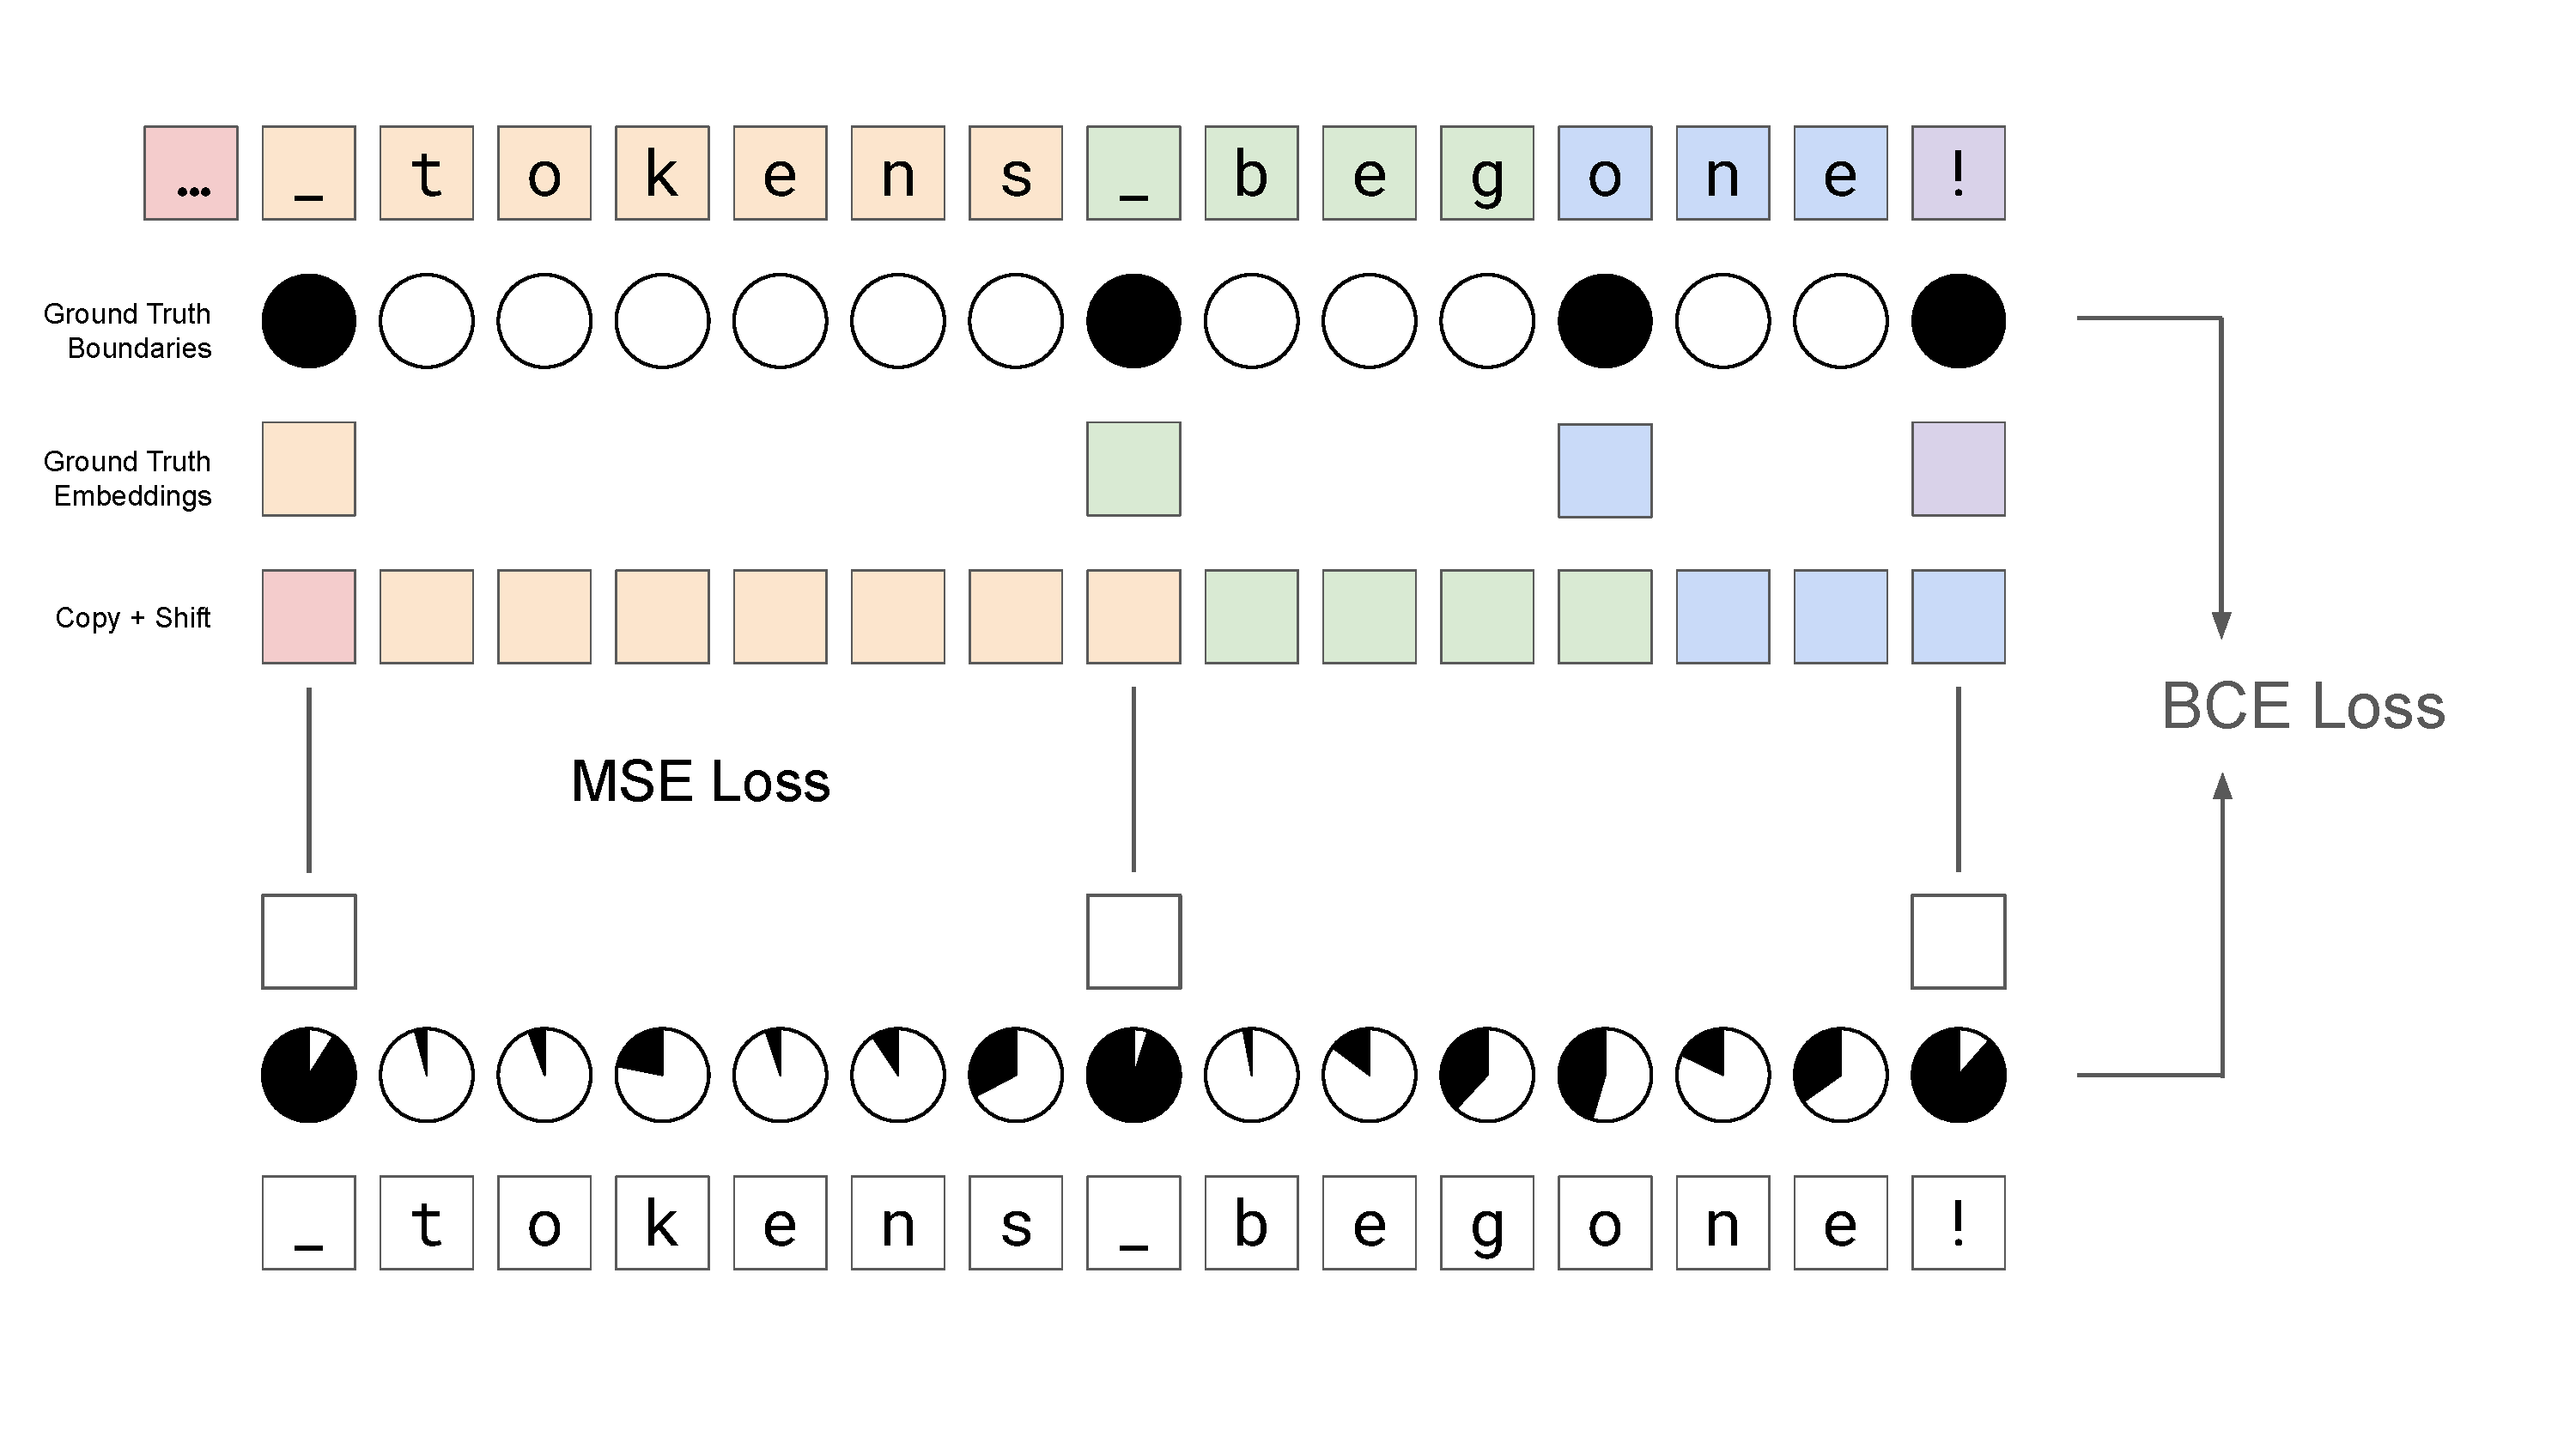
\includegraphics[width=0.7\linewidth]{fig_img/distill.pdf}
\end{center}
\caption{
\textbf{Auxiliary loss strategy for training the encoder} of a \model{} with pretrained main stage. 
In order to mimic the behavior of the tokenizer + embedding layer of a pretrained language model, we add supervision to both the \router{} boundary probabilities
and to the hidden states that we pass through to the \main{}.
These losses encourage the encoder to tokenize once at the start of every token, while also passing the correct embedding into the \main{} near the start of the token,
thus making maximal use of the next-token prediction ability.
}
\label{fig: distill}
\end{figure}